\section{Executed Benchmark Details}
\label{app:benchmarks}

\subsection{Scenario families currently registered}

The current executable benchmark registry contains two kinds of scenarios.

\paragraph{Native synthetic families.}
These are low-cost controlled surrogates used for rapid stability and mechanism checks:
\begin{itemize}
\item \texttt{darcy\_synth} for smoothing-dominant elliptic behavior;
\item \texttt{navier\_stokes\_synth} for mixed transport-diffusion behavior;
\item \texttt{wave\_synth} for packet transport and short-time wavefront motion.
\end{itemize}

\paragraph{Cached PDE families imported from the TCNO artifact.}
These are the larger 192$\times$192 cached scenarios used for the broad PDE benchmark:
\begin{itemize}
\item \texttt{poisson\_robin\_*};
\item \texttt{diffusion\_neumann\_*};
\item \texttt{helmholtz\_dirichlet\_*};
\item \texttt{helmholtz\_impedance\_*};
\item \texttt{helmholtz\_variable\_*};
\item \texttt{helmholtz\_highk\_*};
\item \texttt{helmholtz\_multimodal\_*};
\item \texttt{helmholtz\_partial\_*};
\item evaluation-only OOD rows \texttt{helmholtz\_highk\_ood\_*}.
\end{itemize}

\paragraph{Sequence-valued rollout families.}
These are handled by \codepath{scripts/run\_mino\_long\_rollout.py} rather than by the one-step benchmark runner:
\begin{itemize}
\item \texttt{navier\_stokes\_long\_rollout\_synth}, a deterministic synthetic vorticity rollout for smoke tests;
\item \texttt{navier\_stokes\_long\_rollout\_pino}, an external-cache path for $64\times64$ long temporal Navier--Stokes trajectories.
\end{itemize}
The external cache is intentionally optional. If it is absent, the loader fails with a clear message and the synthetic smoke scenario remains available.

This appendix records a unified executed benchmark contract with scenario metadata, staged campaign profiles, trainable wrapper baselines, and imported mature reference rows.

\subsection{Campaign stages}

The current runner exposes four named campaign stages.

\begin{enumerate}
\item \textbf{Stage 0: smoke sanity.} One seed, two epochs, small subset. Purpose: verify that every loader/model combination remains finite and stable.
\item \textbf{Stage 1: breadth benchmark.} One seed, eight epochs, broad regime matrix. Purpose: determine where MiNO is already strong and where the main gap remains.
\item \textbf{Stage 2: shortlist strengthening.} Three seeds, longer training, theoretically important shortlist. Purpose: attach variance bars to the most important conclusions.
\item \textbf{Stage 3: flagship oscillatory benchmark.} Three seeds, largest local budget, wave plus hard Helmholtz families. Purpose: produce the headline paper table.
\item \textbf{Rollout diagnostic track.} Autoregressive Navier--Stokes rollout at horizons $T=10,20,50$. Purpose: test nonlinear error accumulation and packet-budget drift outside the one-step theorem claim.
\end{enumerate}

The artifact executes Stage~0 fully, executes Stage~1 as a broad one-seed discovery pass, and includes an executed Stage~2 shortlist with three seeds on the most important wave, diffusion, and Helmholtz rows. Stage~3 is the next large compute task.

\subsection{Model roster}

The current executable roster contains:
\begin{itemize}
\item theorem-facing \MiNO-Core;
\item empirical \MiNO-Plus;
\item official-style local wrappers for FNO, Conv-FNO, WNO-style, UNO, and FNO+LearnedLocalTC;
\item imported TCNO reference rows for the same official families on cached PDE scenarios;
\item optional imported DMNO rows for DCR-NO on overlapping retained-law scenarios.
\end{itemize}

This means the appendix can now distinguish three comparison modes:
\begin{enumerate}
\item \MiNO-Core vs.\ \MiNO-Plus;
\item local wrapper compatibility checks on common loaders;
\item mature imported reference baselines on the large cached suites.
\end{enumerate}

\subsection{Current smoke snapshot}

Table~\ref{tab:smokesnapshot} records the executed stage-0 smoke snapshot.

\begin{table}[t]
\centering
\caption{Executed stage-0 smoke snapshot. Lower relative $\ell^2$ is better.}
\label{tab:smokesnapshot}
\begin{tabular}{llll}
\toprule
Scenario & Model & Relative $\ell^2$ & Comment \\
\midrule
\texttt{wave\_synth} & \MiNO-Core & 0.617 & stable theorem-facing core \\
\texttt{wave\_synth} & \MiNO-Plus & 0.492 & improved empirical superset \\
\texttt{helmholtz\_dirichlet\_control} & \MiNO-Core & 0.165 & stable but weak oscillatory baseline \\
\texttt{helmholtz\_dirichlet\_control} & \MiNO-Plus & 0.152 & modest oscillatory gain \\
\texttt{diffusion\_neumann\_control} & \MiNO-Core & 0.0048 & strong smooth-regime result \\
\texttt{diffusion\_neumann\_control} & \MiNO-Plus & 0.0048 & strong smooth-regime result \\
\bottomrule
\end{tabular}
\end{table}

The smoke stage records the first qualitative pattern that persists in the breadth stage: \MiNO-Plus helps most on transport-sensitive scenarios, while the diffusion family is already a genuine strength regime.

\subsection{Current breadth snapshot}

Table~\ref{tab:breadthsnapshot} records a compact subset of the current stage-1 breadth snapshot together with representative mature TCNO references on the same scenario families.

\begin{table}[t]
\centering
\caption{Current breadth snapshot from the executed stage-1 campaign. The imported reference column reports the strongest TCNO-family mean among the mature frozen rows currently merged into the benchmark summaries.}
\label{tab:breadthsnapshot}
\begin{tabular}{p{0.28\textwidth}ccc}
\toprule
Scenario & \MiNO-Core & \MiNO-Plus & Best imported TCNO reference \\
\midrule
\texttt{diffusion\_neumann\_control} & 0.0044 & 0.0045 & 0.0048 (WNO-style) \\
\texttt{diffusion\_neumann\_positive} & 0.0062 & 0.0062 & 0.0054 (WNO-style) \\
\texttt{wave\_synth} & 0.603 & 0.191 & n/a \\
\texttt{helmholtz\_dirichlet\_control} & 0.156 & 0.120 & 0.019 (UNO) \\
\texttt{helmholtz\_dirichlet\_positive} & 0.284 & 0.220 & 0.043 (UNO) \\
\texttt{helmholtz\_variable\_control} & 0.108 & 0.066 & 0.022 (Conv-FNO) \\
\texttt{helmholtz\_highk\_positive} & 0.488 & 0.411 & 0.052 (UNO) \\
\texttt{poisson\_robin\_control} & 0.034 & 0.031 & 0.014 (WNO-style) \\
\bottomrule
\end{tabular}
\end{table}

Table~\ref{tab:breadthsnapshot} is the breadth-stage evidence table. The empirical picture is:
\begin{enumerate}
\item \MiNO-Plus is consistently better than \MiNO-Core on the important oscillatory families.
\item The diffusion family is already competitive with the strongest imported references.
\item The remaining gap is concentrated in the hardest cached Helmholtz suites.
\end{enumerate}

\subsection{Stage-2 shortlist snapshot}

Table~\ref{tab:stage2snapshot} records representative rows from the executed three-seed shortlist. It removes the most important ambiguity in the one-seed breadth pass: the main Core-to-Plus gains persist under seed variation.

\begin{table}[t]
\centering
\caption{Executed stage-2 shortlist snapshot. Entries are mean $\pm$ standard deviation over three seeds. Lower relative $\ell^2$ is better.}
\label{tab:stage2snapshot}
\small
\begin{tabular}{@{}p{0.26\textwidth}p{0.17\textwidth}p{0.17\textwidth}p{0.24\textwidth}@{}}
\toprule
Scenario & \MiNO-Core & \MiNO-Plus & Strong imported reference \\
\midrule
\texttt{wave\_synth} & $0.561\pm0.023$ & $0.157\pm0.003$ & n/a \\
\texttt{diffusion\_neumann\_control} & $0.00423\pm0.00008$ & $0.00436\pm0.00008$ & $0.00481\pm0.00067$ (WNO-style) \\
\texttt{helmholtz\_dirichlet\_control} & $0.153\pm0.0004$ & $0.0626\pm0.0032$ & $0.019\pm0.006$ (UNO) \\
\texttt{helmholtz\_variable\_control} & $0.101\pm0.001$ & $0.0300\pm0.0015$ & $0.022\pm0.003$ (Conv-FNO) \\
\texttt{helmholtz\_highk\_positive} & $0.464\pm0.013$ & $0.391\pm0.009$ & $0.052\pm0.002$ (UNO) \\
\bottomrule
\end{tabular}
\end{table}

\subsection{Wave ablation diagnostic}

Table~\ref{tab:waveablation} reports a deliberately small branch ablation on \texttt{wave\_synth}. It uses one seed and eight epochs as a diagnostic. It separates a real strength from a mechanism gap: the local refinement head is doing substantial work, while the field-only objective weakly exposes transport and symbol errors.

\begin{table}[t]
\centering
\caption{Wave-only ablation diagnostic for \MiNO-Plus on \texttt{wave\_synth}. One seed, eight epochs. Lower relative $\ell^2$ is better.}
\label{tab:waveablation}
\begin{tabular}{lccc}
\toprule
Ablation & Relative $\ell^2$ & Phase error & Packet consistency \\
\midrule
full \MiNO-Plus & 0.1911 & 1.4099 & 1052.6 \\
freeze transport displacement & 0.1911 & 1.4096 & 1049.9 \\
remove transport branch & 0.1913 & 1.4103 & 1037.9 \\
remove symbol branch & 0.1900 & 1.4093 & 1028.2 \\
remove low-frequency residual & 0.1911 & 1.4099 & 1052.1 \\
remove local refinement head & 0.6031 & 1.4316 & 1131.6 \\
\bottomrule
\end{tabular}
\end{table}

\begin{figure}[t]
\centering
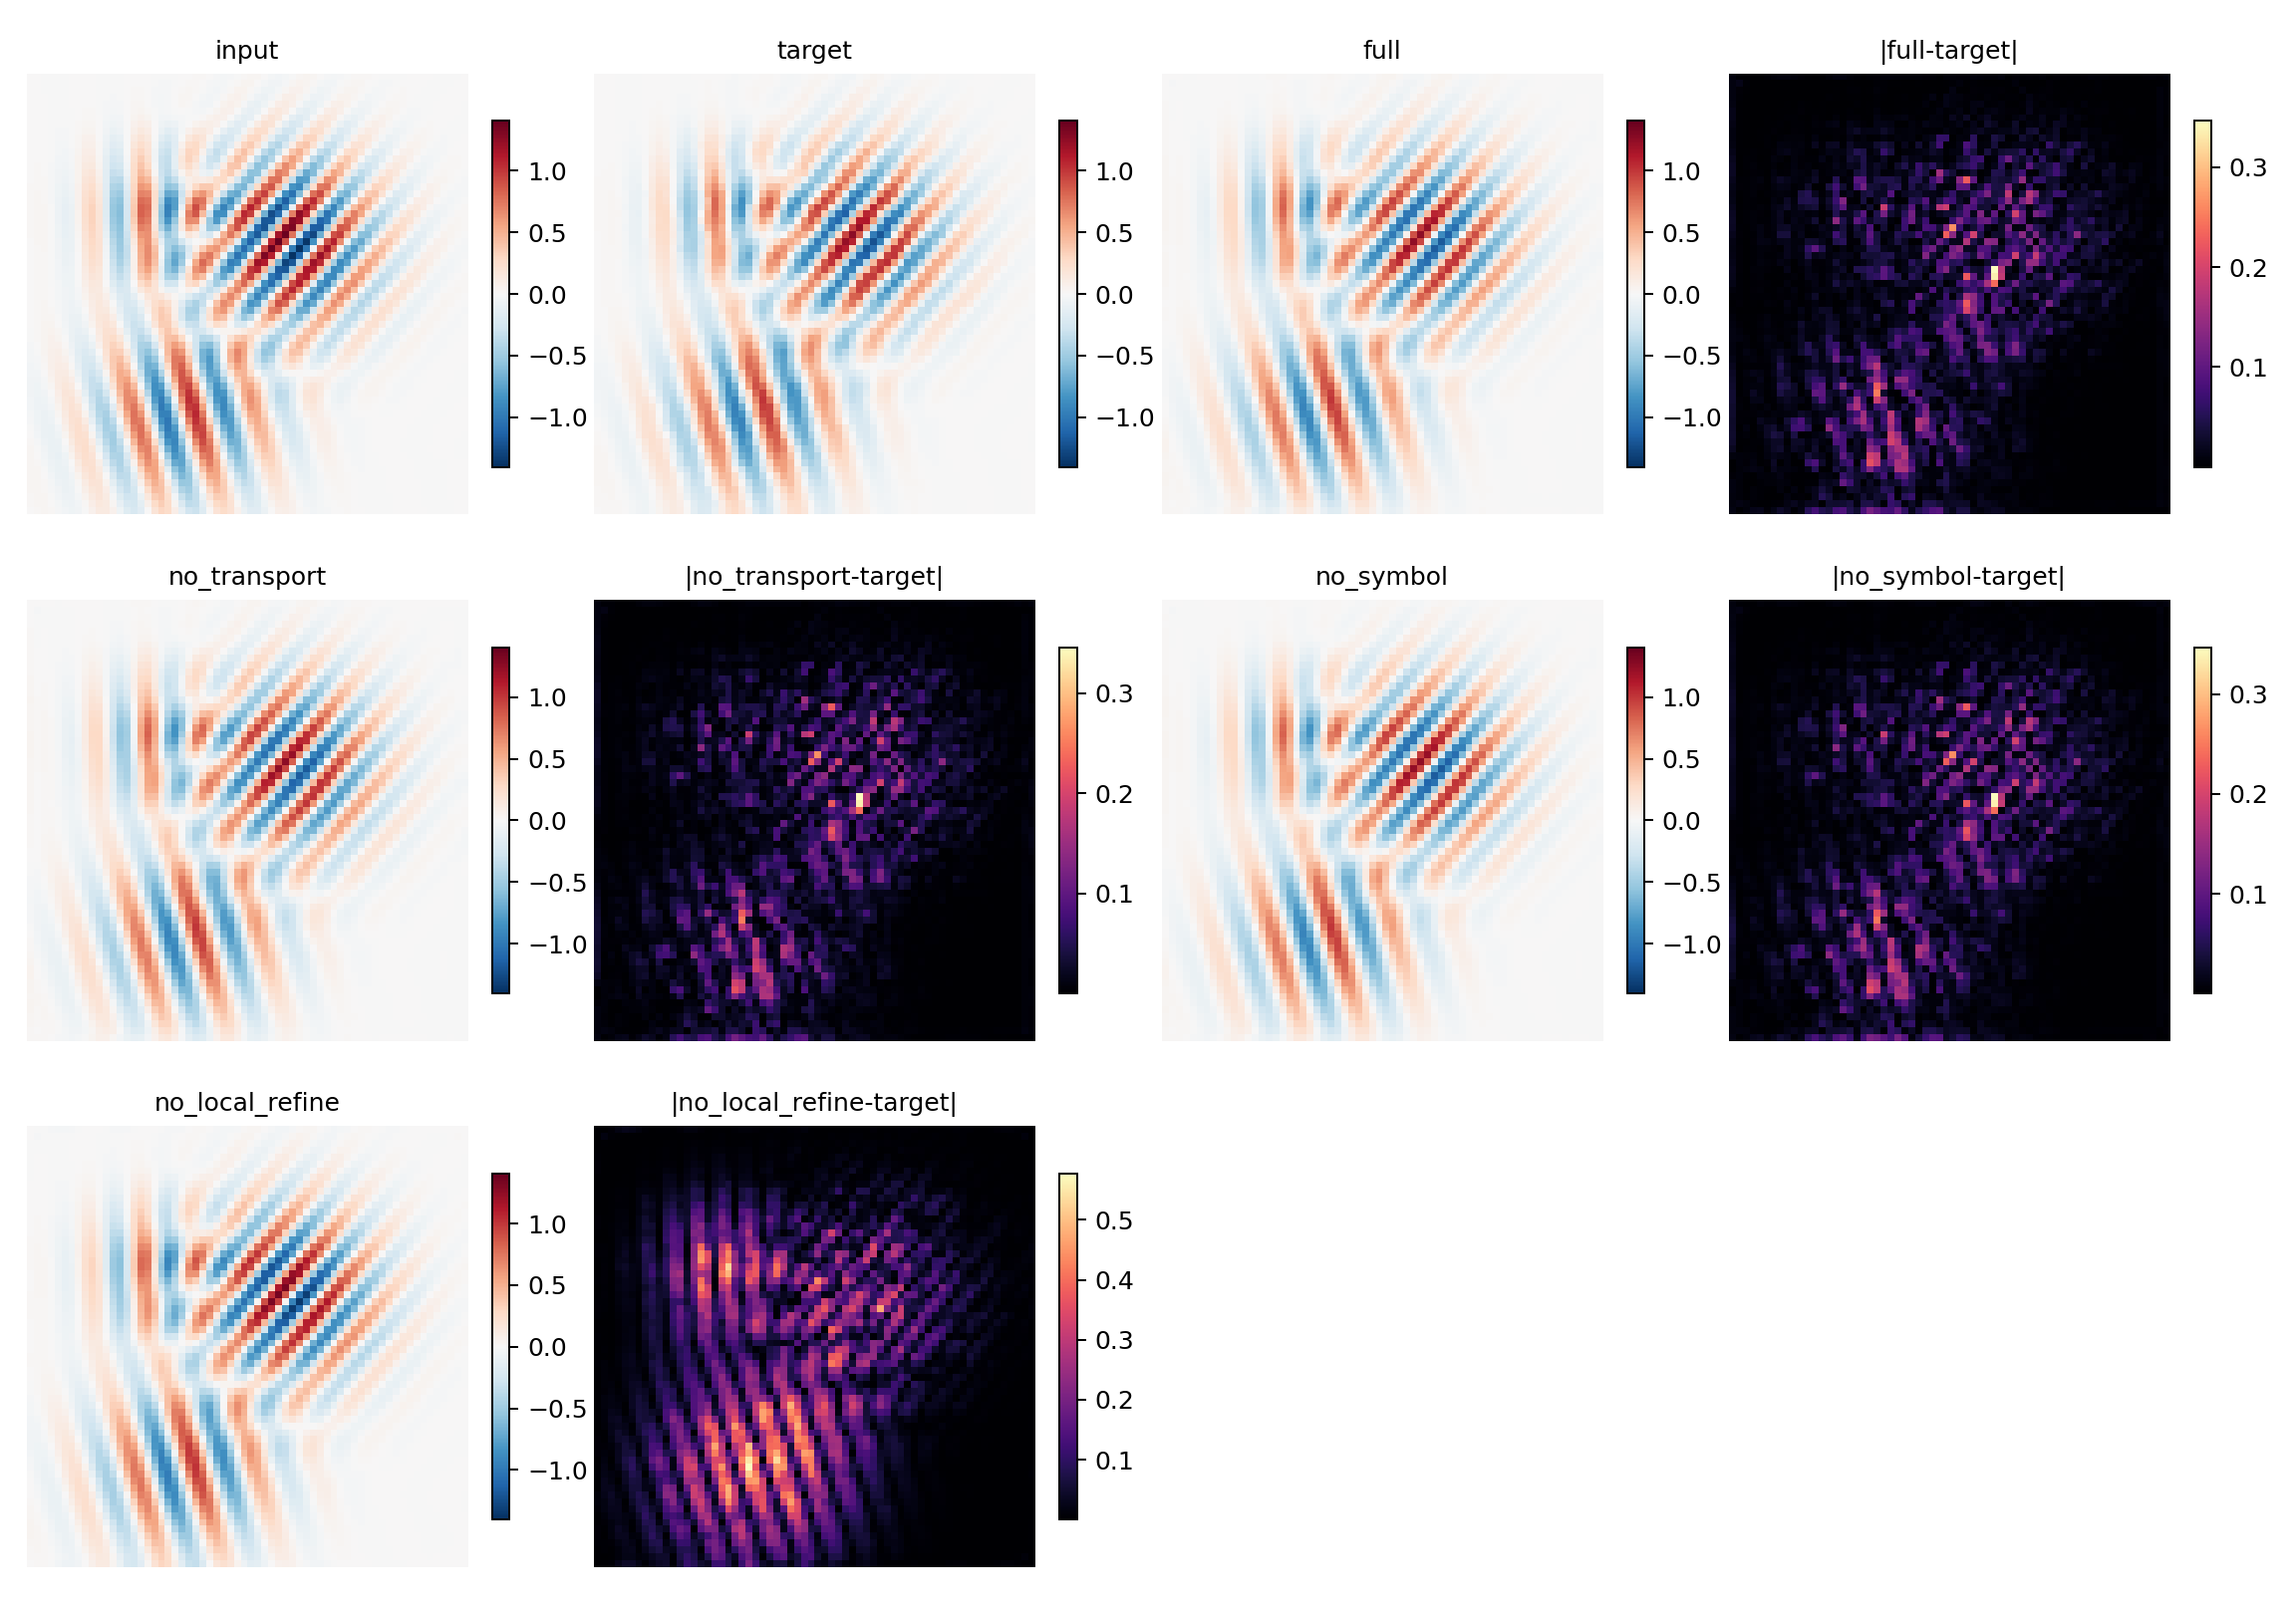
\includegraphics[width=\textwidth]{figures/wave_ablation_prediction.png}
\caption{Wave ablation diagnostic on a held-out \texttt{wave\_synth} example. The figure visualizes the target, full \MiNO-Plus prediction, selected ablated predictions, and absolute error maps. The diagnostic shows that the empirical \MiNO-Plus gain is strongly tied to the local refinement head, while branch-specific transport and symbol effects require sharper proxy losses or longer ablation campaigns to isolate.}
\label{fig:wave-ablation-prediction}
\end{figure}

\subsection{Carrier-bound branch-identifiability campaign}

Table~\ref{tab:branchidv3appendix} records the completed carrier-bound \texttt{branch\_id\_v3} campaign. Each entry is the three-seed mean relative $\ell^2$. The campaign uses \texttt{hamiltonian\_verlet} metadata transport, \texttt{gabor\_gaussian} packetization, sparse top-$K$ aggregation after dense neighbor search, core-first warmup, frozen local refinement during warmup, low-pass released refinement, transported synthesis, transported high-frequency input carrier, canonical proxy loss, symbol-order loss, metadata-flow loss on controlled rows, and same-refinement baseline controls.

The branch labels have the following executable meaning.  \texttt{no\_transport} replaces each propagation block by a zero message and leaves metadata at identity packet centers.  \texttt{identity\_transport} keeps the propagation/message computation but sets displacement to zero; this row is generated by the runner but not displayed in the compact main table.  \texttt{randomized\_metadata} permutes existing metadata across packet tokens before propagation rather than drawing arbitrary phase-space coordinates.  The completed \texttt{branch\_id\_v3\_controls} campaign adds \texttt{no\_transport\_no\_carrier}, which additionally disables transported synthesis and transported input carrier, and \texttt{full\_no\_flow\_supervision}, which sets the effective metadata-flow loss weight to zero while preserving the carrier-bound architecture.  These controls separate three effects: carrier binding, metadata-flow supervision, and learned transport geometry.  The compact controls table is reported in Section~\ref{sec:benchmark-program}; the full raw rows are in \texttt{generated/empirical\_closure/branch\_id\_v3\_controls/}.

\begin{table}[t]
\centering
\caption{Completed carrier-bound \texttt{branch\_id\_v3} relative $\ell^2$ means over three seeds. Lower is better.}
\label{tab:branchidv3appendix}
\small
\begin{tabular}{p{0.26\textwidth}ccccc}
\toprule
Scenario & \MiNO & No transport & Randomized metadata & No symbol & Best same-refine \\
\midrule
\texttt{wave\_bicharacteristic\_control} & 0.380 & 0.714 & 0.912 & 0.395 & 0.056 (UNO) \\
\texttt{wave\_chirp\_propagation} & 0.316 & 0.839 & 1.048 & 0.335 & 0.070 (UNO) \\
\texttt{wave\_two\_packet\_no\_interaction} & 0.204 & 0.777 & 1.037 & 0.236 & 0.022 (UNO) \\
\texttt{wave\_variable\_speed\_nocaustic} & 0.239 & 0.456 & 0.890 & 0.240 & 0.074 (UNO) \\
\texttt{wave\_synth} & 0.295 & 0.537 & 0.900 & 0.298 & 0.154 (UNO) \\
\bottomrule
\end{tabular}
\end{table}

The field-level interpretation is mechanism-positive.  Removing transport consistently degrades relative $\ell^2$, and randomized metadata degrades it further.  On the controlled-flow rows, the full carrier-bound model also has small canonical-flow error, while \texttt{no\_transport} remains at the known-drift error scale and \texttt{randomized\_metadata} is much larger.  The same-refinement UNO baseline is the strongest absolute-error row in every scenario shown in Table~\ref{tab:branchidv3appendix}; the table therefore supports branch identifiability while keeping absolute accuracy as a separate comparison axis.

\paragraph{Post-patch implementation sanity.}
After enforcing the theorem-facing \texttt{spectral\_order} branch as multiplier-only and making the symbol-order proxy differentiable, we ran one low-load sanity row rather than restarting the full campaign.  The row is not used in the aggregate evidence tables.  It verifies that the revised executable path remains finite on \texttt{branch\_id\_v3\_controls}/\texttt{wave\_bicharacteristic\_control}/\texttt{full}/seed~7 under the same carrier-bound profile: relative $\ell^2=0.346$, canonical-flow error $4.42\cdot10^{-5}$, packet-wavefront localization error $0.0326$, and runtime $224$ seconds.  The raw files are written under \codepath{generated/empirical_closure/branch_id_v3_controls_symbol_fix_lowfan/}.  A full three-seed rerun is required before these post-patch values should replace the registered \texttt{branch\_id\_v3\_controls} table.

\paragraph{Low-noise targeted probes.}
We also ran two deliberately small low-noise probes after the reviewer-facing gaps were identified.  These rows use four epochs, three seeds, batch size one, and at most four training examples; they are sanity diagnostics, not registered evidence.  First, on \texttt{wave\_bicharacteristic\_control}/\texttt{full}, the transport parameterizations gave relative $\ell^2$ $0.851\pm0.280$ for \texttt{hamiltonian\_verlet}, $0.883\pm0.334$ for \texttt{hamiltonian\_euler}, and $0.365\pm0.032$ for \texttt{mlp\_displacement}.  This does not support an empirical advantage for the Verlet parameterization at this budget; it only confirms that the runner can now compare the three branches under the same carrier-bound protocol.  Second, on \texttt{diffusion\_neumann\_control}, the calculus-regime probe gave relative $\ell^2$ $0.00654\pm0.00067$ for \texttt{full} and $0.00637\pm0.00012$ for \texttt{no\_symbol}.  This does not identify the symbol branch at this budget, consistent with the claim that identity/dissipative symbol attribution needs a proper calculus-regime campaign rather than a deliberately tiny low-load row.

\subsection{Synthetic official-wrapper comparison}

Table~\ref{tab:synthofficial} records the current 16-epoch local comparison on the synthetic families using the official-style wrapper models.

\begin{table}[t]
\centering
\caption{Synthetic official-wrapper comparison at 16 epochs. Lower relative $\ell^2$ is better.}
\label{tab:synthofficial}
\begin{tabular}{p{0.24\textwidth}p{0.22\textwidth}cc}
\toprule
Scenario & Model & Relative $\ell^2$ & Runtime (s) \\
\midrule
\texttt{darcy\_synth} & \MiNO-Core & 0.9989 & 13.8 \\
\texttt{darcy\_synth} & Conv-FNO & 0.9994 & 4.5 \\
\texttt{darcy\_synth} & FNO & 1.0008 & 3.5 \\
\texttt{darcy\_synth} & UNO & 1.0014 & 7.2 \\
\midrule
\texttt{navier\_stokes\_synth} & \MiNO-Plus & 0.9432 & 24.6 \\
\texttt{navier\_stokes\_synth} & Conv-FNO & 0.8647 & 4.6 \\
\texttt{navier\_stokes\_synth} & UNO & 0.8751 & 7.0 \\
\texttt{navier\_stokes\_synth} & WNO-style & 0.8911 & 8.2 \\
\midrule
\texttt{wave\_synth} & \MiNO-Plus & 0.1807 & 24.5 \\
\texttt{wave\_synth} & UNO & 0.1868 & 7.2 \\
\texttt{wave\_synth} & Conv-FNO & 0.2204 & 4.4 \\
\texttt{wave\_synth} & WNO-style & 0.4322 & 8.2 \\
\bottomrule
\end{tabular}
\end{table}

The synthetic comparison has a simple interpretation. MiNO trails the best official wrappers on the synthetic Navier--Stokes surrogate, while the empirical enlargement is close to the best synthetic wave wrappers. The Darcy row is a low-cost sanity check because all models cluster near relative $\ell^2\approx 1$.

\subsection{Interpreting the executed numbers}

The breadth snapshot is a one-seed, eight-epoch discovery pass and is read for \emph{pattern}.

\paragraph{Strong evidence present.}
The model split is empirically meaningful, the theorem-facing core and the empirical superset are both stable, and there is at least one clear strength regime in the cached PDE suite.

\paragraph{Hard-regime evidence gate.}
The hardest oscillatory cached suites favor the mature imported baselines by large factors. Multi-seed shortlist, branch-identifiability, and flagship oscillatory campaigns are the evidence gate for any backbone-level dominance claim.

\subsection{Metric panel actually produced by the runner}

The executed runner already records:
\begin{itemize}
\item relative $\ell^2$ field error;
\item phase error;
\item packet-consistency score;
\item runtime and parameter count;
\item imported top-$k$ capture when frozen TCNO references are merged.
\end{itemize}

This metric panel is narrower than the final ideal microlocal dashboard, but it is already aligned with the theorem-aware decomposition. Relative $\ell^2$ remains the headline number, while phase error and packet consistency carry the transport-sensitive interpretation.

The long-rollout runner records a wider diagnostic panel:
\begin{itemize}
\item mean and final rollout relative $\ell^2$;
\item rollout stability;
\item spectral energy error and high-frequency energy drift;
\item enstrophy error for scalar-vorticity trajectories;
\item empirical packet budgets \texttt{transport\_budget}, \texttt{symbol\_budget}, and \texttt{residual\_budget};
\item packet trajectory, amplitude, residual-energy, and cascade diagnostics.
\end{itemize}
These metrics are written to raw JSON, aggregate CSV, and dry-run plan CSV files. The raw rows are preserved so that interrupted campaigns can be resumed without overwriting previous results.

\subsection{Scientific value of the snapshot}

The appendix records a strictly stronger empirical state:
\begin{enumerate}
\item a unified executable benchmark registry;
\item stable theorem-facing and empirical MiNO models;
\item imported mature reference baselines on the cached PDE families;
\item a broad one-seed discovery pass that separates strength regimes from stress regimes.
\end{enumerate}

These rows support disciplined empirical claims about where the microlocal primitive helps and where engineering and optimization remain active.
